
\title{Research Summary}
%\date{\today}

\documentclass[12pt]{report}
\usepackage{amsmath,amsxtra,amssymb,latexsym, amscd,amsthm}
\usepackage{url}
\usepackage{color}
\usepackage[mathscr]{eucal}
\usepackage{amsfonts}
\usepackage{graphicx}
\usepackage{fancybox}
\usepackage{multirow}
\usepackage{multicol}
\usepackage{array}
\usepackage[autostyle]{csquotes}
\usepackage{balance}
\usepackage[nottoc]{tocbibind}
\usepackage{float}
\usepackage{geometry}
\usepackage{lipsum}
\usepackage[utf8]{inputenc}
\geometry{ a4paper, total={210mm,297mm},  left=20mm, right=20mm,  top=20mm, bottom=20mm }

\newcolumntype{L}[1]{>{\raggedright\let\newline\\\arraybackslash\hspace{0pt}}m{#1}}
\newcolumntype{C}[1]{>{\centering\let\newline\\\arraybackslash\hspace{0pt}}m{#1}}
\newcolumntype{R}[1]{>{\raggedleft\let\newline\\\arraybackslash\hspace{0pt}}m{#1}}
\newcommand\tab[1][1cm]{\hspace*{#1}}
\renewcommand{\bibname}{References}

\begin{document}
	
	\thispagestyle{empty}
	\begin{center}
		
		\vspace*{3cm}
		{\bf \LARGE PROJECT REPORT}\\
		\vspace*{2cm}
		Topic:\\
		{\bf \Large Project topic}\\
		\vspace{3cm}
		{\Large University of Information Technology}\\
		\vspace{5cm}
		%{\Large DOAN DUY}\\
		{\Large June 2020}
	\end{center}
	%\thispagestyle{empty}
	
	\newpage
	\vspace*{5cm}
	\begin{center}
		{\bf \Large Student Information}\\
		Student name: \tab Student ID:\\
		Student 1 \tab 18520XXX\\
		Student 2 \tab 18520AAA\\
		\vspace{5cm}
		{\bf \Large Supervisor}\\
		Supervisor's name
	\end{center}
	
%	\frontmatter
	\newpage
	%%%%%%%%%%%%%%%%%%%%%%%%%%%%%%%%%%%%%%%%%%%
%+ Acknowledgment
%+ Revised: 13-07-2016
%+ Last revised: 24-07-2016
%%%%%%%%%%%%%%%%%%%%%%%%%%%%%%%%%%%%%%%%%%%
\section*{\centering{Acknowledgments}}
%\addcontentsline{toc}{chapter}{Acknowledgements}
Here is your acknowledgment.
Please giving your thanking to all people who have support or contribution to your work.


\begin{flushright}
Here is your name.
\end{flushright}

%%%%%%%%%%%%%%%%%%%%%%%%%%%%%%%%%%%%%%%%%%%
%+ End of Acknowledgment
%%%%%%%%%%%%%%%%%%%%%%%%%%%%%%%%%%%%%%%%%%%
	
	\tableofcontents
	\listoffigures
	\listoftables
	%\pagenumbering{arabic}
	\chapter{Introduction}
	\section{Review}
	Listing related works here.
	The related works can be papers published at a conference or on journal.
	When you cite to these works,
	please use the IEEE reference format.
	For example,
	Earlier Deadline First (EDF) \cite{ref10} is one of the most popular scheduling algorithms on uniprocessor system.
	
	You also refer to some website.
	When doing so,
	please select proper and original one and use citation like \cite{ref1}.
	
	
	Then, give your comments on these works: what is advantage? What is disadvantage?
	By evaluating related works, 
	you can emphasise the reason why you conduct the project.
	
	\section{Ojectives}
	
	Stating your objectives here. What do you want to achieve after the project?
	\begin{itemize}
		\item Ojective 1.
		\item Ojective 2.
		\item ...
	\end{itemize}
	
	\section{Expected results}
	Description of the product, simulation, or any other kind of results
	that you expect to achieve.
	
	\section{Scope/Limitation}
	State clearly what you will do, what will not do...
	
	\chapter{Work description}
	
	In this chapter, you should describe clearly your design.
	The content should include the following things:
		
	\section{System description}
	This section includes the system design with schematic diagram.
	The schematic shows all components of the design and internal connections.
	You need to describe the meaning/feature/requirement of every component
	and the type/interface of connections.	
	
	When you insert any figure into the report,
	you must give references to the figure somewhere and
	have explanation of the figure.
	For instance,
	Figure \ref{fig:systemdesign} shows the system design of the fingering-locked door.
	The system consists of eight main components: power supply, fingering reader,...
	The power supply is a 3 V DC.
	...
	The fingering reader connect to computer using SPI connection with the speed of...
	
	\begin{figure}[ht]
		\begin{center}
			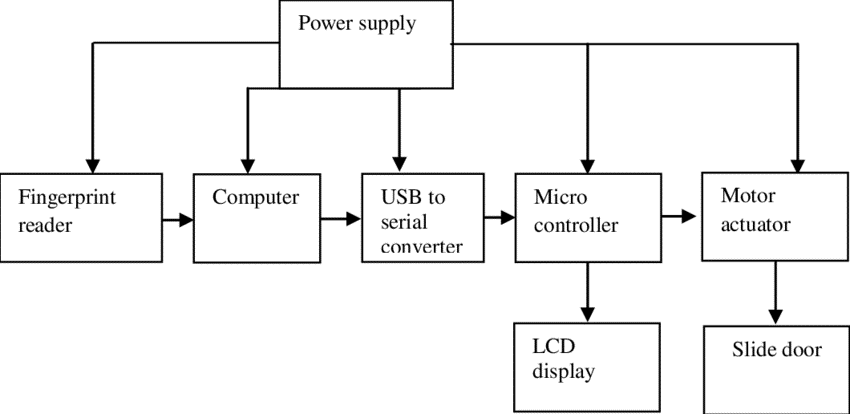
\includegraphics[width=\textwidth]{SystemDesign.png}
			\caption{System design of the fingering-lock door}\label{fig:systemdesign}
		\end{center}
	\end{figure}
	
	
	
	\section{Operating flow}
	This section describes the operating flow for each feature of your design.
	Operating flow shows the processing steps of the feature from the power on to the result showing.
	It also includes how people interact and use the feature provided.
	
	For example,
	Figure \ref{fig:operatingflow} shows the operating flow of the automatic watering feature.
	Then, you should describe the processing flow on the figure.
	Each feature is required for at least one operating flow.
	
	\begin{figure}[ht]
		\begin{center}
			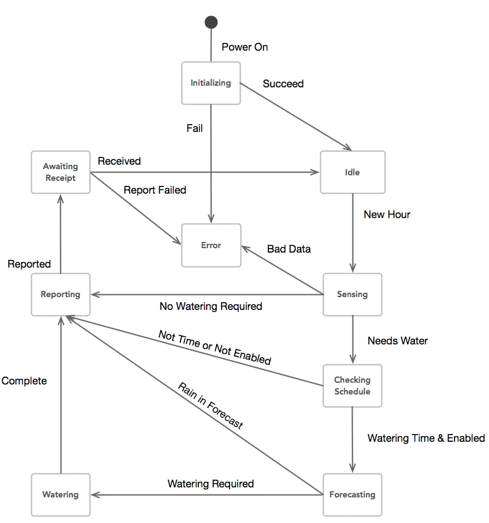
\includegraphics[width=\textwidth]{OperatingFlow.png}
			\caption{Operating flow of the automatic watering feature}\label{fig:operatingflow}
		\end{center}
	\end{figure}
	
	Besides,
	you may you some equations in your report.
	The equations can be inserted into the report and referred in text.
	See the following example: 
	
	Let $eS_i(t)$ denote the resources (the number of time slots) 
	that $\tau_i$ is entitled to receive by time $t$ under the proportionate scheduling.
	Then, the resources requested by task $\tau_i$ is calculated as: 
	
	\begin{equation} \label{eS}
	eS_i(t) = \lfloor \mu_i*t \rfloor
	\end{equation}
	
	\chapter{Results}
	This chapter shows your achievement and discussion for the whole work.
	
	\section{Achievement}
	This section is listing all results that you achieve after finishing the project.
	You must compare with the objectives to clarify which is done and which is not done.
	
	If you use some table, please give description in detail including meaning of each column, row and then comments on results.
	For example, see the following table and its description.
	
	\begin{table}[h]
		\renewcommand{\arraystretch}{1.3}
		\caption{Results of scheduler invocation}
		\label{tb::invocation}
		\begin{center}
			\begin{tabular}{|c|C{1cm}|C{2cm}|C{1cm}|C{1cm}|C{1cm}|}
				\hline
				\multirow{2}{2cm}{No. of processor}&\multirow{2}{1cm}{Up (\%)}&\multirow{2}{2cm}{No. of instance}&\multicolumn{3}{c|}{No. of scheduler invocation}\\
				\cline{4-6}
				& & &{\bf LAA}&{\bf Pfair}&{\bf RUN}\\
				\hline
				\multirow{5}{1cm}{4}&{60}&{4117}&\multirow{5}{1cm}{1000}&\multirow{5}{1cm}{10000}&{3955}\\
				\cline{2-3}\cline{6-6}
				{}&{70}&{4701}&{}&{}&{3726}\\
				\cline{2-3}\cline{6-6}
				{}&{80}&{4402}&{}&{}&{3806}\\
				\cline{2-3}\cline{6-6}
				{}&{90}&{2269}&{}&{}&{2077}\\
				\cline{2-3}\cline{6-6}
				{}&{100}&{3969}&{}&{}&{3743}\\
				\hline
				\multirow{5}{1cm}{32}&{60}&{19209}&\multirow{5}{1cm}{1000}&\multirow{5}{1cm}{10000}&{7953}\\
				\cline{2-3}\cline{6-6}
				{}&{70}&{22909}&{}&{}&{8368}\\
				\cline{2-3}\cline{6-6}
				{}&{80}&{29111}&{}&{}&{8657}\\
				\cline{2-3}\cline{6-6}
				{}&{90}&{34359}&{}&{}&{8998}\\
				\cline{2-3}\cline{6-6}
				{}&{100}&{33931}&{}&{}&{8868}\\
				\hline
			\end{tabular}
		\end{center}
	\end{table}
	
	Table \ref{tb::invocation} shows the average number of scheduler invocation for three examined algorithms.
	On the table,
	the first column is the number of processors;
	the second one is the task utilizations;
	the third one shows the number of instance released within the observation period; and
	the last three columns show results for LAA, Pfair, and RUN, respectively.
	As multiples of ten,
	tasks' period decides intervals of ten in length for the LAA algorithm.
	Consequently,
	the LAA scheduler is invoked 1000 times over 10000 ticks of observation.
	Pfair, meanwhile,
	results in 10000 times
	because the scheduler is invoked at every tick.
	Results of RUN are better than those of Pfair,
	but worse than those of LAA.
	Obviously,
	LAA is the best on the criterion of scheduler invocation.
	
	\section{Difficulties}
	Listing difficulties (if any) you are faced with during the work.
	
	\section{Discussion}
	Give your discussion about the possibility of expanding/improving your project.
	Give more example applications possible for your design.
	
	\newpage
	\begin{thebibliography}{1}
	\bibitem{ref1}
	Li, Y., Liu, H., Wu, Q., Mu, F., Yang, J., Gao, J., Li, C., \& Lee, Y. J. (2023). GLIGEN: Open-Set Grounded Text-to-Image Generation. In Proceedings of the IEEE/CVF Conference on Computer Vision and Pattern Recognition (CVPR) (pp. 22511-22521).
\end{thebibliography}
\end{document}